%=========================================
\subsection{Additional Plots}
This section provides additional plots illustrating the performance of the experiments.

Figure~\ref{fig:q_throughput_16} shows the measured throughput,
as images per second, delivered by each system for all queries and databases.
In comparison to figure~\ref{fig:q_throughput_56}, when using fewer concurrent 
clients (nthr = 16), the throughput for VDMS for queries \textit{q4} (\textit{2tag\_or\_resize}), 
\textit{q5} (\textit{2tag\_resize\_geo\_and}), and
\textit{q6} (\textit{2tag\_resize\_geo\_or}) improved by a large margin 
for the 50M and 100M databases. 
In the case of \textit{q4} and \textit{q6}, the throughput for 50M (and 100M for \textit{q4})
increase by a large margin which outperforms both baselines while, in figure~\ref{fig:q_throughput_56},
PostgreSQL slightly performed better than VDMS. 
In the case of \textit{q5}, all systems perform a little differently for databases
larger than 5M.  The gaps between the throughput of each system narrows at 10M.  
At a database size of 50M, the performance of the baselines drastically drop
while the throughput of VDMS has a large improvement in comparison.

\begin{figure}[ht]
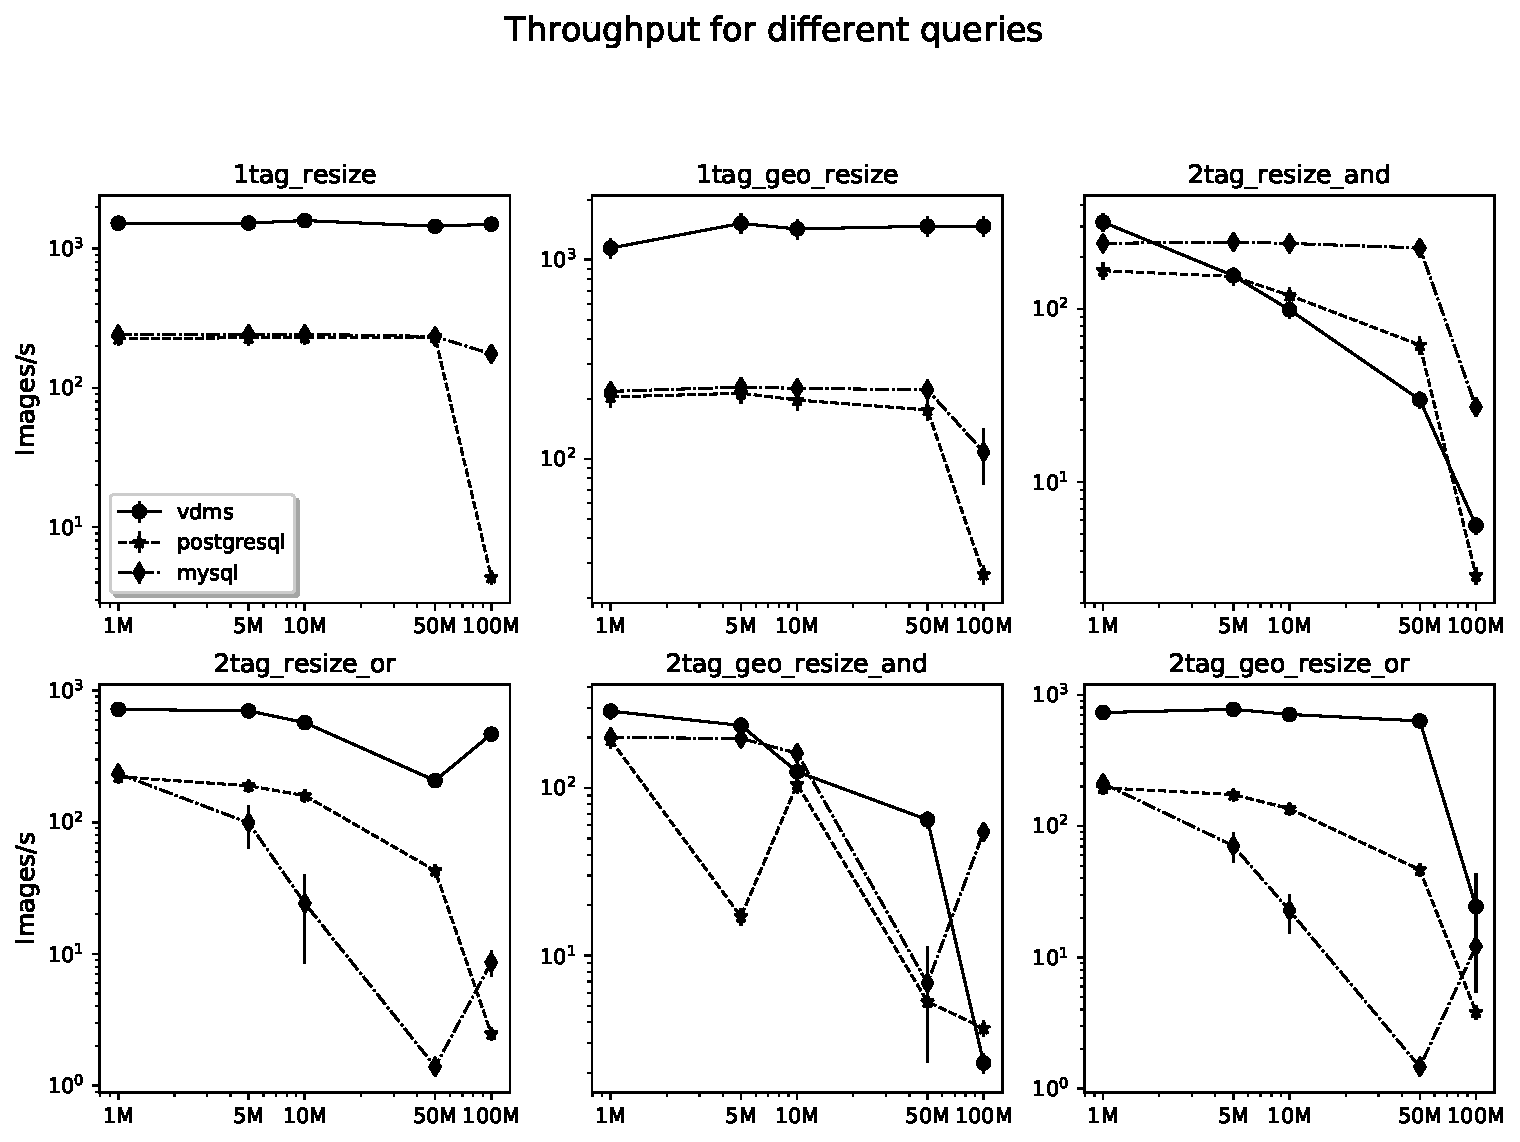
\includegraphics[width=\columnwidth]{figures/plot_th_16_mosaic_results_throughput}
\caption{Throughput Analysis using all queries from our use-case
described in the Experimental Setup Section.
We show queries in different figures for readability reasons.
The experiments show the performance of all systems (VDMS and the two baselines) as the
database size increases.
These queries were run using 16 simultaneous clients (nthr = 16),
and averaged out of 5 runs.}
\label{fig:q_throughput_16}
\end{figure}

Figure~\ref{fig:summary_mysql} summarizes the results
comparing VDMS and MySQL. We see up to 96x speedup (for the case of \textit{q2}),
and an average improvement in throughput of about 31x.
We also see how \textit{q3} and \textit{q5} have poor performances and scalability
as the database size grows, same as shown in Figure~\ref{fig:summary_postgresql}.
Considering all other queries (\textit{q1}, \textit{q2}, \textit{q4}, and \textit{q6}), 
VDMS provides at least 3x speedup in throughput.

\begin{figure*}[ht]
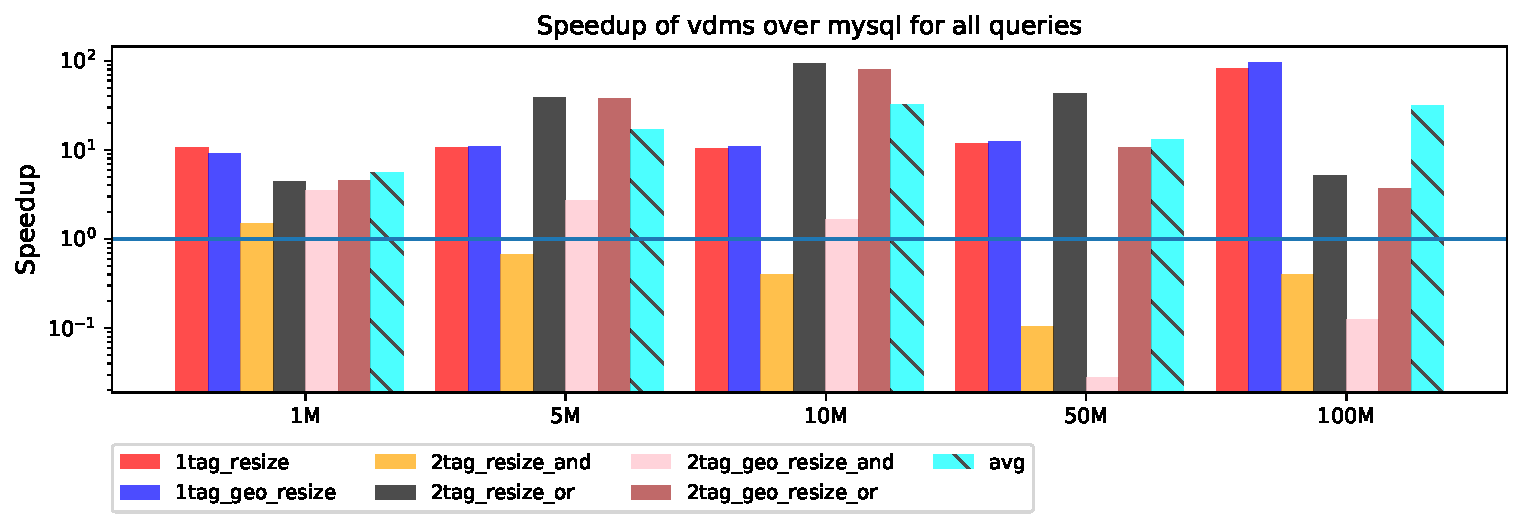
\includegraphics[width=\textwidth]{figures/plot_th_56_query_times_speedup_mysql}
\caption{Summary of performance gains for all queries.
We see up to 96x speedup (\textit{q2}), and an average of about 31x.
More importantly, we see that the speedup grow as the database size increases,
showing that VDMS scales better than the MySQL baseline.}
\label{fig:summary_mysql}
\end{figure*}
%=========================================
